\documentclass[12pt, fleqn]{article}

%%% FONTS AND MATH %%%
\usepackage{amsmath}
\usepackage{amsfonts}
\usepackage[english]{babel}
\usepackage{bbm} %%% Indicators

%%% VERBATIM INPUT %%%
\usepackage{fancyvrb}
\usepackage{dcolumn,graphicx,amsmath,amssymb,algorithm,algpseudocode,physics}
\usepackage{hyperref}
\usepackage{modiagram}
\usepackage[fleqn]{mathtools}
\setlength{\mathindent}{1cm}

%%% IMAGES %%%
\usepackage{graphicx}
\graphicspath{ {./} }
\usepackage{hyperref}

%%% SOURCE CODE %%%
\usepackage{listings}
\usepackage{color}
\usepackage{multicol}
\usepackage[compress,numbers]{natbib}
 
\definecolor{codegreen}{rgb}{0,0.6,0}
\definecolor{codegray}{rgb}{0.5,0.5,0.5}
\definecolor{codepurple}{rgb}{0.58,0,0.82}
\definecolor{backcolour}{rgb}{0.95,0.95,0.92}
 
\lstdefinestyle{mystyle}{
    backgroundcolor=\color{backcolour},   
    commentstyle=\color{codegreen},
    keywordstyle=\color{magenta},
    numberstyle=\tiny\color{codegray},
    stringstyle=\color{codepurple},
    basicstyle=\footnotesize,
    breakatwhitespace=false,         
    breaklines=true,                 
    captionpos=b,                    
    keepspaces=true,                 
    numbers=left,                    
    numbersep=5pt,                  
    showspaces=false,                
    showstringspaces=false,
    showtabs=false,                  
    tabsize=2
}
 
\lstset{style=mystyle}

%%% MARGINS %%%
\usepackage[left=1in, right=1in, top=1in, bottom=1in]{geometry}

%%% HEADERS %%%
\usepackage{fancyhdr}
\pagestyle{fancy}
\rhead{ \textbf {Yu, Jimmy} \\ \url{https://github.com/jkyu} }
\lhead{}

\begin{document}
\section*{The Davidson Subspace Method}
\subsection*{Summary}
\label{subsec:Summary}
The Davidson method, also called ``Davidson-Liu'' or ``Block Davidson'' or some combination of those terms, is a subspace method for obtaining the smallest (or largest) eigenvalues and their associated eigenvectors for a given matrix.
The need for such a method arises when it is unnecessary to solve the standard eigenvalue decomposition problem, which simultaneously yields all of the eigenvalues and eigenvectors. 
For instance, one may be interested in only several eigenvectors (e.g., as part of principal component analysis), and performing the full matrix decomposition may feel unnecessary. \newline

\noindent The Davidson method has become a ubiquitous part of electronic structure algorithms as the means by which the electronic Schr\"odinger equation is solved in order to obtain low-lying eigenstates of the system. 
The full Hamiltonian matrix for even moderately-sized molecular systems can require hundreds of gigabytes (or more!) of storage, rendering direct eigendecomposition (or even explicit computation of the Hamiltonian itself) computationally intractable under most circumstances.
The Davidson method was in fact developed for this very purpose by Ernest Davidson in 1978 \cite{Davidson1983}.
The following will be a brief dive into the theory behind the method. 

\subsection*{The subspace eigenvalue problem}
Suppose we have a square matrix $\mathbf{A} \in \mathbb{R}^{n \times n}$ for which we want the lowest eigenvalues, $\{\lambda_i\}$, and their associated eigenvectors, $\{u_i\}$. 
That is:
\begin{align}
    \mathbf{A} u_i = \lambda_i u_i 
\end{align}
For whatever reason (computational limitations, efficiency, etc.), we would like to solve for $\{\lambda_i\}$ and $\{u_i\}$ without performing an eigendecomposition directly. 
We will proceed by solving the eigenvalue problem within a subspace spanned by some orthonormal basis $\{v_j\}$, which populate the columns of a matrix $\mathbf{V} \in \mathbb{R}^{n \times m}$, where $m$ is the number of vectors in the basis set $\{v_j\}$ and $n$ is the dimension the matrix $\mathbf{A}$. \newline

\noindent Let $\tilde{\mathbf{A}}$ be the projection of $\mathbf{A}$ in the subspace spanned by $\{v_i\}$. 
Solving for the eigenvectors of $\tilde{\mathbf{A}}$ yields:
\begin{align}
    \tilde{\mathbf{A}} \tilde{u}_i = \tilde{\lambda}_i \tilde{u}_i
\end{align}
where
\begin{align}
    \tilde{u}_i = \sum_j c_{ij} v_j = \mathbf{V} c_i
\end{align}
That is, $\tilde{u}_i$ can be expressed as a linear combination of the basis vectors $\{v_j\}$ with coefficients $c_{ij}$.
Alternatively, this can be expressed as a matrix-vector product between the coefficient vector $c_i$ and the matrix $\mathbf{V}$.
The true eigenvector $u_i$ is therefore approximated by $\tilde{u}_i$ obtained via eigendecomposition of $\mathbf{A}$ projected into the subspace $\mathbf{V}$. 

\subsection*{The orthogonal residuals}
What can be done with this approximation to $u_i$?
Consider a quantity $r_i$ defined as:
\begin{align}
    r_i \equiv \mathbf{A} \tilde{u}_i - \tilde{\lambda}_i \tilde{u}_i
\end{align}
This is some residual resulting from the approximate nature of $\tilde{u}_i$. 
If $\tilde{u}_i = u_i$, the residual would be exactly zero. 
Under the assumption that $\tilde{u}_i$ is the best possible approximation to $u_i$ within the subspace $\mathbf{V}$, the accuracy of the approximation is limited by the subspace itself.
Then components outside of $\{v_j\}$ are required in order to more accurately approximate $u_i$ and reduce the residual $r_i$. 
In other words, the residual is orthogonal to the subspace $\mathbf{V}$: 
\begin{align}
    r_i \equiv (\mathbf{A} \tilde{u}_i - \tilde{\lambda}_i \tilde{u}_i) \perp \{v_j\}
\end{align}
The main idea behind the Davidson method derives from this orthogonality condition.
In order to obtain the best approximation $\tilde{u}_i$ to $u_i$, the residual $r_i$ must be minimized.
The Davidson method approaches this by augmenting the subspace $\mathbf{V}$ with basis vectors that were ``missing'' from $\{v_j\}$ and then solving the subspace eigenvalue problem again in the augmented subspace.
The assumption is that this ``missing'' information is contained in the residual vector $r_i$. 
By iteratively solving the subspace eigenvalue problem and augmenting the subspace, $\tilde{u}_i$ eventually converges to $u_i$.
In the worst case, this requires reaching the point where $\tilde{\mathbf{A}} = \mathbf{A}$, i.e., where $\{v_j\}$ has expanded to the point where $\mathbf{A} \in \text{span}(\{v_j\})$.
Needless to say, the worst case is worse than having directly attempted the eigendecomposition of $\mathbf{A}$. 


\subsection*{The Davidson algorithm}
Now with some intuition behind the method, we can proceed to a description of the algorithm and a representation of the method in quantities that are amenable to code.
From equations (3) and (5), we obtain the following relationship due to orthogonality:
\begin{align}
    &r_i^* \mathbf{V} = (\mathbf{A} \tilde{u}_i - \tilde{\lambda}_i \tilde{u}_i)^* \mathbf{V} = 0 \\
    &\implies \tilde{u}_i^* \mathbf{A}^* \mathbf{V} - \tilde{\lambda}_i \tilde{u}_i^* \mathbf{V} = 0 \\
    &\implies \tilde{u}_i^* \mathbf{A}^* \mathbf{V} = \tilde{\lambda}_i \tilde{u}_i^* \mathbf{V} \\
    &\implies (\mathbf{V} c_i)^* \mathbf{A}^* \mathbf{V} = \tilde{\lambda}_i (\mathbf{V} c_i)^* \mathbf{V} \\
    &\implies c_i^* \mathbf{V}^* \mathbf{A}^* \mathbf{V} = \tilde{\lambda}_i c_i^* \mathbf{V}^* \mathbf{V} \\
    &\implies c_i^* \mathbf{V}^* \mathbf{A}^* \mathbf{V} = \tilde{\lambda}_i c_i^* \\
    &\implies \mathbf{V}^* \mathbf{A} \mathbf{V} c_i = \tilde{\lambda}_i c_i 
\end{align}
where equation (11) follows from the orthonormality of $\mathbf{V}$, i.e., $\mathbf{V}^* \mathbf{V} = \mathbf{I}$, and equation (12) results from take the complex conjugate of both sides of equation (11). 
Notice that equation (12) is the subspace eigenvalue problem solved at each step of the iterative Davidson process, as $\tilde{\mathbf{A}} = \mathbf{V}^* \mathbf{A} \mathbf{V}$ is exactly the projection of $\mathbf{A}$ into the subspace $\mathbf{V}$. 
Rewriting this more compactly yields:
\begin{align}
    \tilde{\mathbf{A}} c_i = \tilde{\lambda}_i c_i 
\end{align}
Diagonalizing $\tilde{\mathbf{A}}$ yields $c_i$ and $\tilde{\lambda}_i$, and $\tilde{u}_i$ can be obtained from equation (3).
The residual $r_i$ can then be computed as:
\begin{align}
    r_i = \mathbf{A} \mathbf{V} c_i - \tilde{\lambda}_i \mathbf{V} c_i
\end{align}
$r_i$ can then be appended to $\mathbf{V}$ and the next iteration can proceed with a more complete subspace.
Once $r_i \approx 0$ according to some error metric ($l_2$ error being a simple one), $\mathbf{V}$ essentially includes all basis vectors of $\mathbf{A}$ necessary to fully describe the eigenvector $u_i$. \newline

\noindent A few considerations before writing down the recipe for the Davidson algorithm: 
\begin{itemize}
    \item It is often desirable to work with an orthonormal basis set at each step. This can be done by orthonormalizing the subspace basis set $\{v_j\}$ after it is expanded. A QR decomposition or an explicit Gram-Schmidt procedure can easily achieve this. However, it has recently been reported that orthogonalization without normalization may accelerate convergence via a ``balancing'' process \cite{Parrish2016}.
    \item A subspace for the initial projection of $\mathbf{A}$ is required. The basis vectors that comprise this set are often termed "trial vectors." For diagonally dominant spatially sparse matrices, the unit basis vectors may be an appropriate choice. For some applications, a more more physically motivated choice may make sense, e.g., a Davidson method implemented for configuration interaction may employ unit vectors ordered according to Koopman energies. Proper selection of trial vectors can have an impact on the rate of convergence.
    \item Often in electronic structure codes, the Hamiltonian matrix is not explicitly computed and stored. Instead of projecting the Hamiltonian into the subspace, the matrix-vector product $\sigma = \mathbf{A} \mathbf{V} \tilde{\mathbf{u}}$ is formed directly in the subspace. 
    \item Additionally, a variety of preconditioning techniques may accelerate the convergence and improve the stability of the Davidson iterations. 
\end{itemize}

\noindent Without further delay, the Davidson algorithm can be summarized as follows:
\begin{algorithm}
\caption{Davidson-Liu algorithm for obtaining extreme eigenvalues and their corresponding eigenvectors}
\begin{algorithmic}[1]
    \Procedure{Davidson-Liu}{$\mathbf{A}$, $n_{\text{evecs}}$, convergence\_threshold}
        \State Form orthonormal set of trial vectors $\{v_j\}$ for the initial subspace $\mathbf{V}$
        \While{max(\{norm($r_i$)\}) $<$ convergence\_threshold}
            \State Orthonormalize the subspace basis vectors
            \State Project $A$ into the subspace: 
                $ \tilde{\mathbf{A}} = \mathbf{V}^* \mathbf{A}^* \mathbf{V} $
            \State Solve the subspace eigenvalue problem:
                $ \tilde{\mathbf{A}} c_i = \tilde{\lambda}_i c_i $
            \State Compute the set of residuals $\{r_i\}$ for each desired eigenvector: 
                $ r_i = \mathbf{A} \mathbf{V} c_i - \tilde{\lambda}_i \mathbf{V} c_i $
            \State Append the set of residuals $\{r_i\}$ to the subspace basis $\{v_j\}$
        \EndWhile 
    \EndProcedure
\end{algorithmic}
\end{algorithm}


\subsection*{Accelerating computation of eigenvalues and eigenvectors}
Although the Davidson algorithm was developed for application to Hamiltonian diagonalization by quantum chemists for configuration interaction problems, it can also accelerate eigenvalue/eigenvector computation in other matrix problems for which only a handful of eigenvectors must be obtained.
An obvious example from data science is principal component analysis (PCA). 
This is a method that takes data as input and determines vectors of maximum variance, reducing high dimensional data to several axes, the principal components, that attempt to summarize factors that determine variance in the data. 
Often, only 1-3 vectors are chosen to represent these axes so as to be easily visualized. 
The PCA can be interpreted as a rotation into the frame of the eigenvectors of a covariance matrix followed by a dimensionality reduction onto the subset of eigenvectors one wishes to retain. 
Since only a small number of eigenvectors are desired, the Davidson can be used to obtain these without incurring the full cost of explicit diagonalization of the covariance matrix. 
This is advantageous for extremely large data sets, as the eigenproblem is the computational bottleneck of a standard PCA.
Davidson is by no means the only approach to doing so -- a variety of Krylov subspace methods, e.g., the Lanczos algorithm, may be used to achieve a similar result. 

First, we examine the computational performance of the Davidson on routine eigensolves. \autoref{fig:dav-scaling} summarizes the computational scaling on rank-sparse (\textsf{rank==10}) but spatially dense matrices of varying sizes. 
The Davidson demonstrates apparent linear scaling, which may save significant time for large matrices when compared to a full eigensolve performed by the naive application of NumPy's \textsf{linalg.eigh()} routine \cite{numpy}.
Similarly, the maximum eigenvalue and eigenvector errors per Davidson solve are extremely low relative to traditional computation via NumPy, as can be observed by the y-axis scaled by $10^{-8}$ (\autoref{fig:dav-error}).  

Next, we examine the acceleration afforded by implementation of the Davidson routine in a kernel PCA.
The kernel PCA is used instead in cases for which the data of interest is not linearly separable \cite{Scholkopf1998}.
The data is first mapped to a high dimensional space in which the data can now be linearly separated.
This is called the kernel trick.
The identity of the kernel is often swept under the rug, but a popular example is the Gaussian radial basis function, which is just a Gaussian that takes the Euclidean distance between two points as an argument. 
The kernel returns a scalar value that implicit encodes information about the high dimensional space, allowing the construction of the ``kernel'' matrix, a proxy for the covariance matrix.
Diagonalization of principal components that may allow for the linear separation of data that previously had no obvious separating hyperplane. 
One complication of the kernel PCA is that good performance of the kernel depends on proper selection of parameters that may need to be specified for the kernel function.
This necessitates parameter optimization as a part of data analysis with kernel methods.

A summary of the results can be observed in \autoref{fig:kpca-scaling}. 
The dataset is generated using the \textsf{make\_moons} function from scikit-learn \cite{scikit}, which generates data in two crescent shapes that cannot be cleanly separated by a linear hyperplane. 
This is a popular example set for demonstrating the kernel trick. 
The Davidson significantly reduces the time required to solve the eigenvalue problem; however, for kernel PCA, the bottleneck at systems of these sizes is in formation of the kernel matrix. 
By employing the Davidson, the cost of the kernel PCA is almost entirely the cost of forming the kernel matrix. 


\begin{figure}[ht]
\centering
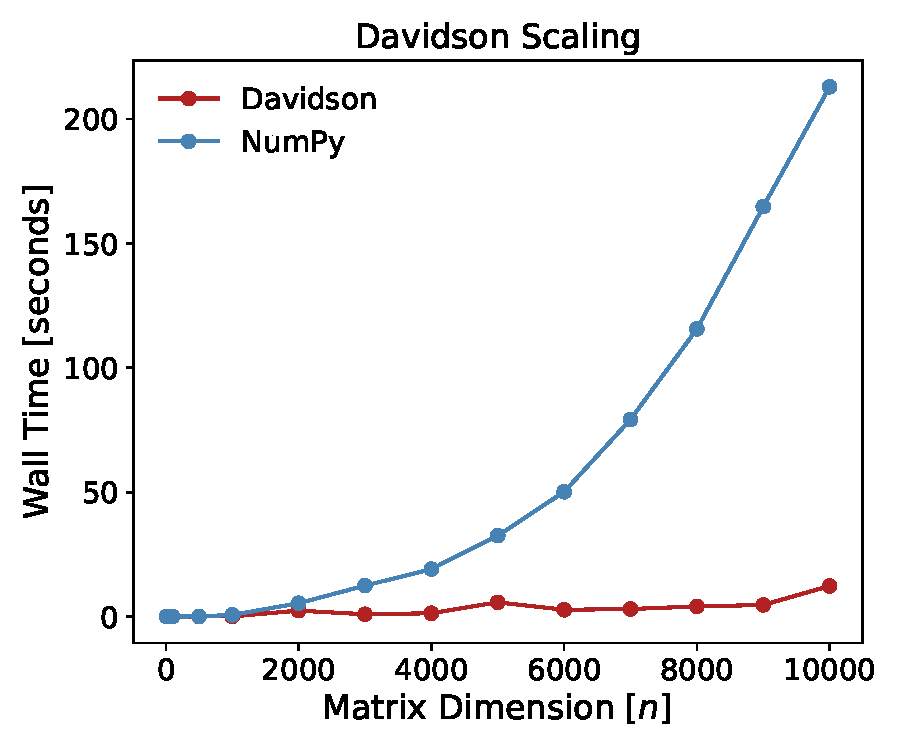
\includegraphics[width=\textwidth]{./figures/dav_scaling.pdf}
\caption{
Scaling of the Davidson versus NumPy's linalg.eigh routine for diagonalization of rank sparse (\textsf{rank==10}) but spatially dense matrices of a variety of dimensions.
The Davidson algorithm yields apparent linear scaling for obtaining low-lying eigenvectors, avoiding the full $O(N^3)$ computational cost of full diagonalization. 
}
\label{fig:dav-scaling}
\end{figure}


\begin{figure}[ht]
\centering
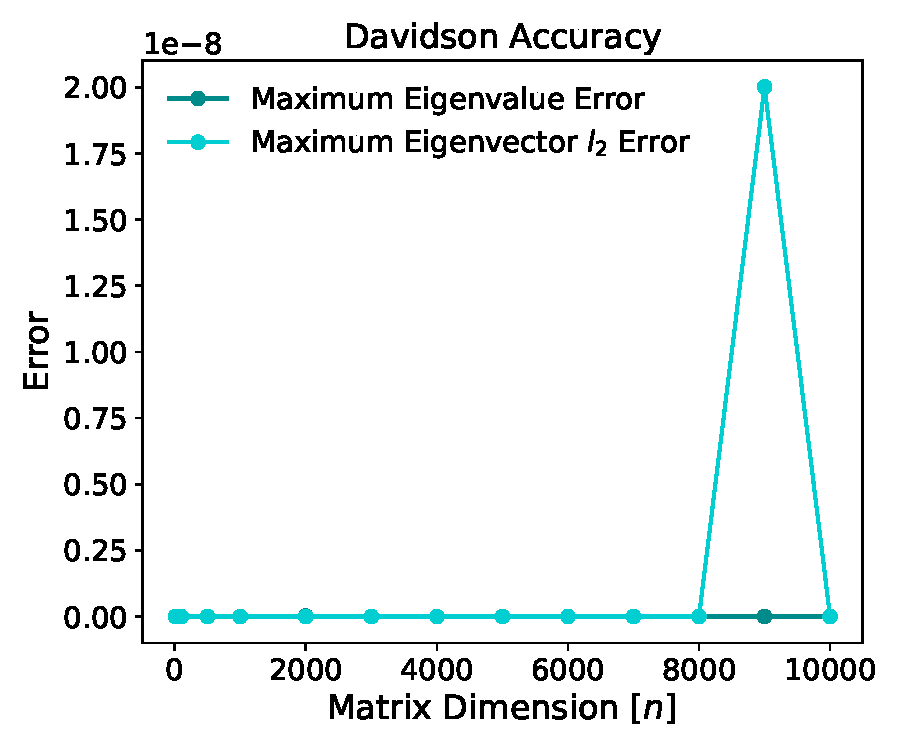
\includegraphics[width=\textwidth]{./figures/dav_error.pdf}
\caption{
Maximum $l_2$ error among all eigenvectors and maximum absolute error among all eigenvalues obtained using the Davidson method. 
These errors are almost negligible, with the maximum error computed to be on the order of $10^{-8}$. 
}
\label{fig:dav-error}
\end{figure}


\begin{figure}[ht]
\centering
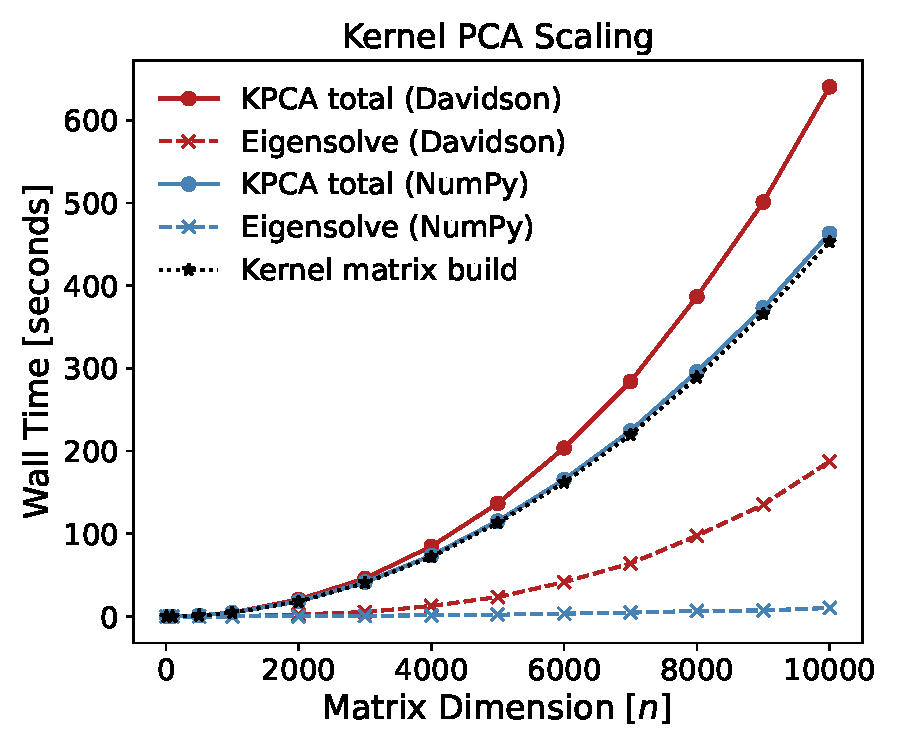
\includegraphics[width=\textwidth]{./figures/kpca_scaling.pdf}
\caption{
Scaling of the Davidson versus NumPy's linalg.eigh routine for kernel PCA. 
Implementation of the Davidson reduces the computational expense of the eigensolve portion of a kernel PCA.
Unfortunately, the formation of the kernel matrix is the bottleneck here.
}
\label{fig:kpca-scaling}
\end{figure}



\newpage
\bibliographystyle{plain}
\bibliography{references}

\end{document}
